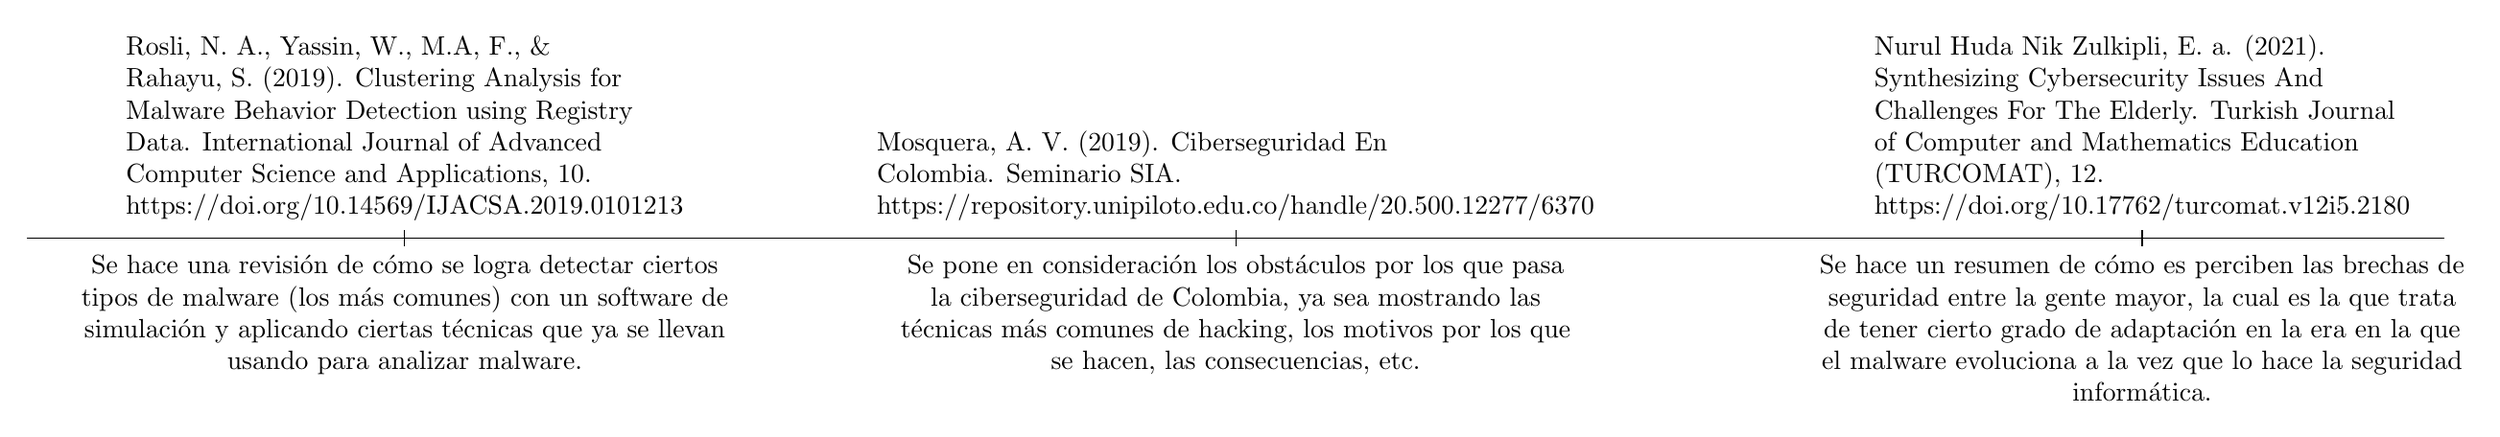
\begin{tikzpicture}
% draw nodes to add events
\draw (0,0) -- (32,0);
% draw vertical lines
\foreach \x in {5,16,28}
\draw (\x cm,3pt) -- (\x cm,-3pt);

% draw nodes to add events
\draw (5,0) node[below=3pt, align=center] {
  Se hace una revisión de cómo se logra detectar ciertos \\
  tipos de malware (los más comunes) con un software de \\
  simulación y aplicando ciertas técnicas que ya se llevan \\
  usando para analizar malware.
} 
node[above=3pt, align=left] {
  Rosli, N. A., Yassin, W., M.A, F., \& \\
  Rahayu, S. (2019). Clustering Analysis for \\
  Malware Behavior Detection using Registry \\
  Data. International Journal of Advanced \\
  Computer Science and Applications, 10. \\
  https://doi.org/10.14569/IJACSA.2019.0101213
};
\draw (16,0) node[below=3pt, align=center] {
  Se pone en consideración los obstáculos por los que pasa \\
  la ciberseguridad de Colombia, ya sea mostrando las \\
  técnicas más comunes de hacking, los motivos por los que \\
  se hacen, las consecuencias, etc.
} node[above=3pt, align=left] {
  Mosquera, A. V. (2019). Ciberseguridad En \\
  Colombia. Seminario SIA. \\
  https://repository.unipiloto.edu.co/handle/20.500.12277/6370
};
\draw (28,0) node[below=3pt, align=center] {
  Se hace un resumen de cómo es perciben las brechas de \\
  seguridad entre la gente mayor, la cual es la que trata \\
  de tener cierto grado de adaptación en la era en la que \\
  el malware evoluciona a la vez que lo hace la seguridad \\
  informática.
} node[above=3pt, align=left] {
  Nurul Huda Nik Zulkipli, E. a. (2021). \\
  Synthesizing Cybersecurity Issues And \\
  Challenges For The Elderly. Turkish Journal \\
  of Computer and Mathematics Education \\
  (TURCOMAT), 12. \\
  https://doi.org/10.17762/turcomat.v12i5.2180
};
\end{tikzpicture}

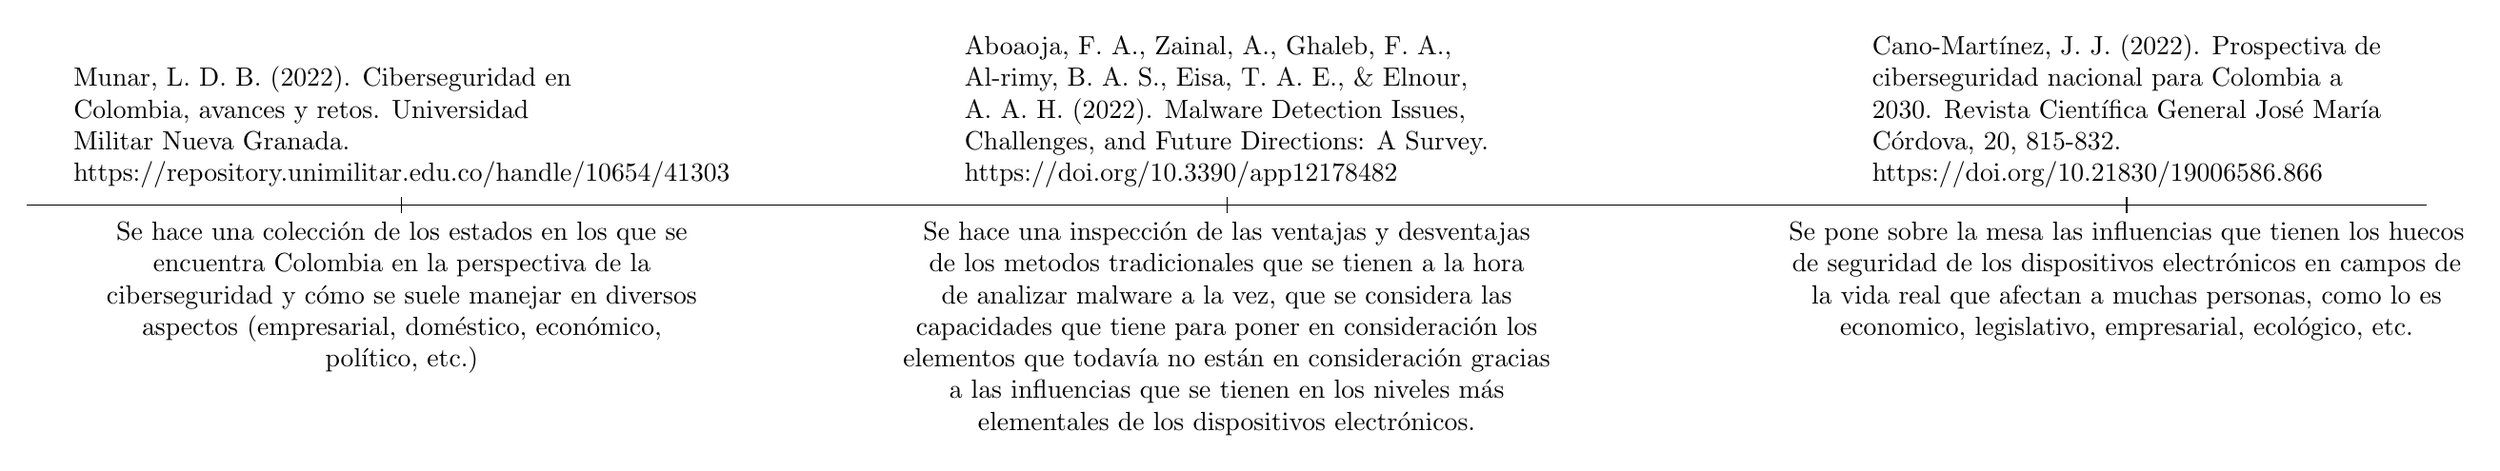
\begin{tikzpicture}
% draw nodes to add events
\draw (0,0) -- (32,0);
% draw vertical lines
\foreach \x in {5,16,28}
\draw (\x cm,3pt) -- (\x cm,-3pt);

% draw nodes to add events
\draw (5,0) node[below=3pt, align=center] {
  Se hace una colección de los estados en los que se \\
  encuentra Colombia en la perspectiva de la \\
  ciberseguridad y cómo se suele manejar en diversos \\
  aspectos (empresarial, doméstico, económico, \\
  político, etc.)
} node[above=3pt, align=left] {
  Munar, L. D. B. (2022). Ciberseguridad en \\
  Colombia, avances y retos. Universidad \\
  Militar Nueva Granada. \\
  https://repository.unimilitar.edu.co/handle/10654/41303
};
\draw (16,0) node[below=3pt, align=center] {
  Se hace una inspección de las ventajas y desventajas \\
  de los metodos tradicionales que se tienen a la hora \\
  de analizar malware a la vez, que se considera las \\
  capacidades que tiene para poner en consideración los \\
  elementos que todavía no están en consideración gracias \\
  a las influencias que se tienen en los niveles más \\
  elementales de los dispositivos electrónicos.
} 
node[above=3pt, align=left] {
  Aboaoja, F. A., Zainal, A., Ghaleb, F. A., \\
  Al-rimy, B. A. S., Eisa, T. A. E., \& Elnour, \\
  A. A. H. (2022). Malware Detection Issues, \\
  Challenges, and Future Directions: A Survey. \\
  https://doi.org/10.3390/app12178482
};
\draw (28,0) node[below=3pt, align=center] {
  Se pone sobre la mesa las influencias que tienen los huecos \\
  de seguridad de los dispositivos electrónicos en campos de \\
  la vida real que afectan a muchas personas, como lo es \\
  economico, legislativo, empresarial, ecológico, etc.
} node[above=3pt, align=left] {
  Cano-Martínez, J. J. (2022). Prospectiva de \\
  ciberseguridad nacional para Colombia a \\
  2030. Revista Científica General José María \\
  Córdova, 20, 815-832.\\
  https://doi.org/10.21830/19006586.866
};
\end{tikzpicture}

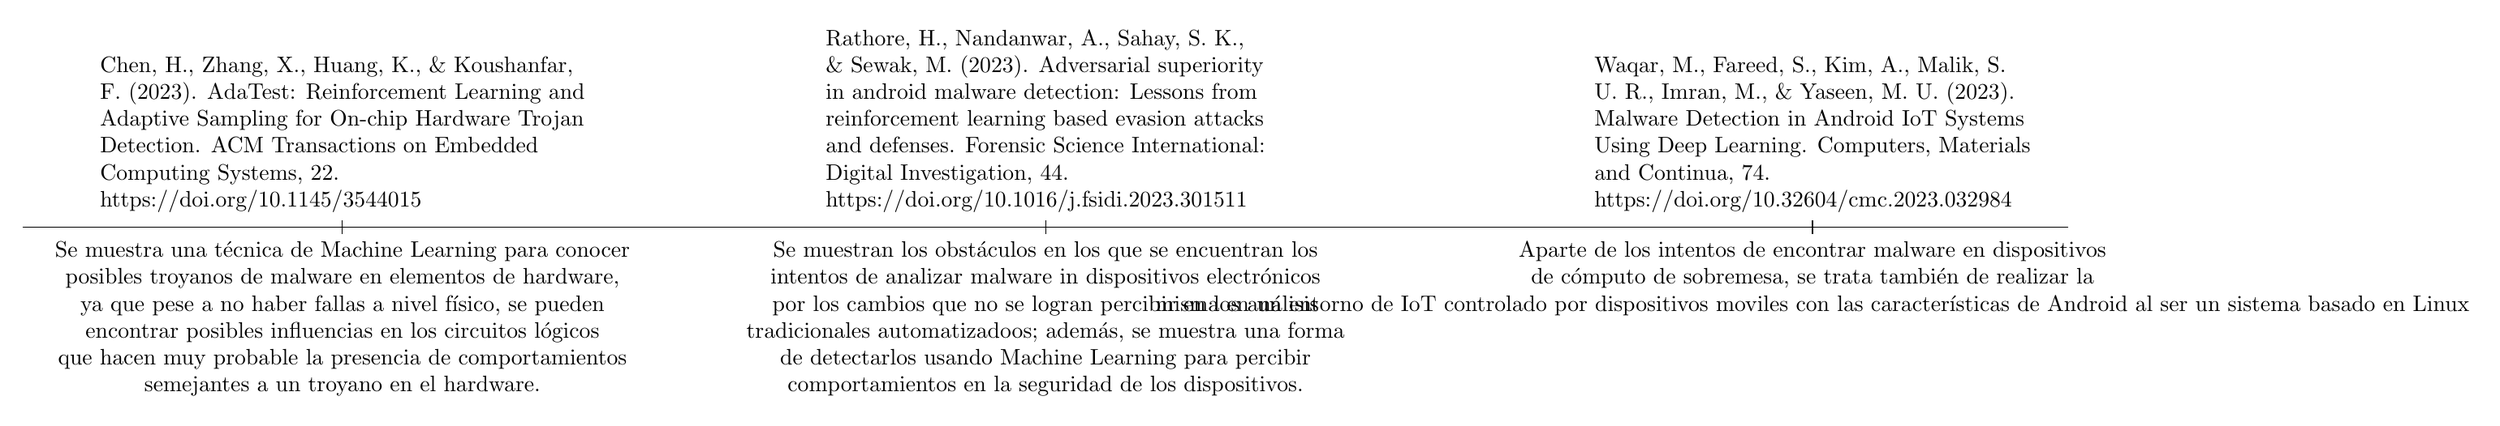
\begin{tikzpicture}
% draw nodes to add events
\draw (0,0) -- (32,0);
% draw vertical lines
\foreach \x in {5,16,28}
\draw (\x cm,3pt) -- (\x cm,-3pt);

% draw nodes to add events
\draw (5,0) node[below=3pt, align=center] {
  Se muestra una técnica de Machine Learning para conocer \\
  posibles troyanos de malware en elementos de hardware, \\
  ya que pese a no haber fallas a nivel físico, se pueden \\
  encontrar posibles influencias en los circuitos lógicos \\
  que hacen muy probable la presencia de comportamientos \\
  semejantes a un troyano en el hardware.
} node[above=3pt, align=left] {
  Chen, H., Zhang, X., Huang, K., \& Koushanfar, \\
  F. (2023). AdaTest: Reinforcement Learning and \\
  Adaptive Sampling for On-chip Hardware Trojan \\
  Detection. ACM Transactions on Embedded \\
  Computing Systems, 22. \\
  https://doi.org/10.1145/3544015
};
\draw (16,0) node[below=3pt, align=center] {
  Se muestran los obstáculos en los que se encuentran los \\
  intentos de analizar malware in dispositivos electrónicos \\
  por los cambios que no se logran percibir en los análisis \\
  tradicionales automatizadoos; además, se muestra una forma \\
  de detectarlos usando Machine Learning para percibir \\
  comportamientos en la seguridad de los dispositivos.
} node[above=3pt, align=left] {
  Rathore, H., Nandanwar, A., Sahay, S. K., \\
  \& Sewak, M. (2023). Adversarial superiority \\
  in android malware detection: Lessons from \\
  reinforcement learning based evasion attacks \\
  and defenses. Forensic Science International: \\
  Digital Investigation, 44.\\
  https://doi.org/10.1016/j.fsidi.2023.301511
};
\draw (28,0) node[below=3pt, align=center] {
  Aparte de los intentos de encontrar malware en dispositivos \\
  de cómputo de sobremesa, se trata también de realizar la \\
  misma en un entorno de IoT controlado por dispositivos moviles con las características de Android al ser un sistema basado en Linux
} node[above=3pt, align=left] {
  Waqar, M., Fareed, S., Kim, A., Malik, S. \\
  U. R., Imran, M., \& Yaseen, M. U. (2023). \\
  Malware Detection in Android IoT Systems \\
  Using Deep Learning. Computers, Materials \\
  and Continua, 74.\\
  https://doi.org/10.32604/cmc.2023.032984
};
\end{tikzpicture}
